\section{Phân tích mã nguồn có lỗ hổng bảo mật}

Theo báo cáo đến năm 2023, tổng cộng có 17 thể loại bug được báo cáo về RUSTSEC Database \cite{zheng2023closer}.
Trong đó, lỗi về an toàn bộ nhớ và đa luồng chiếm tới gần hai phần ba tổng số loại lỗi.
Mặc dù Rust có các cơ chế để khắc phục những lỗi này, nhưng dường như trong những dự án thực tế phức tạp, vẫn tồn tại một số lỗi nhất định, đặc biệt khi sử dụng tính năng \texttt{unsafe} (mã không an toàn) của Rust.
Để minh họa cho việc áp dụng đồ thị CPG vào thực tế, khóa luận sẽ trình bày ứng dụng của đồ thị CPG trên 4 lỗi trong RUSTSEC Database thuộc các thể loại lỗi phổ biến nhất.

\subsection{RUSTSEC-2021-0086}

RUSTSEC-2021-0086 là lỗi về khởi tạo bộ nhớ không an toàn.
Lỗi này xảy ra khi sử dụng hàm \texttt{Vec::with\_capacity} để khởi tạo một vectơ với dung lượng được định sẵn, sau đó sử dụng hàm \texttt{set\_len} để điều chỉnh độ dài của vectơ.
Tuy nhiên hàm \texttt{set\_len}, một hàm được coi là \texttt{unsafe}, nó không khởi tạo giá trị cho các phần tử của vectơ mà chỉ sửa lại độ dài của vectơ, dẫn đến việc các phần tử có giá trị là không xác định.
Để sửa lỗi, ta có thể sử dụng macro \texttt{vec!} để khởi tạo vectơ với độ dài và dung lượng là $N$, giá trị mặc định của mỗi phần tử là $0$.

\begin{listing}[H]
\begin{minted}[mathescape, breaklines, frame=lines, framesep=2mm, baselinestretch=1.2, fontsize=\footnotesize, linenos]{rust}
const N: usize = 255;

// Before fix
let mut buf: Vec<u8> = Vec::with_capacity(N);
unsafe { buf.set_len(N) };

// After fix
let mut buf: Vec<u8> = vec![0; N];
\end{minted}
\caption{Ví dụ mã nguồn cho RUSTSEC-2021-0086}
\label{code:c4_RUSTSEC-2021-0086}
\end{listing}

\begin{figure}[H]
    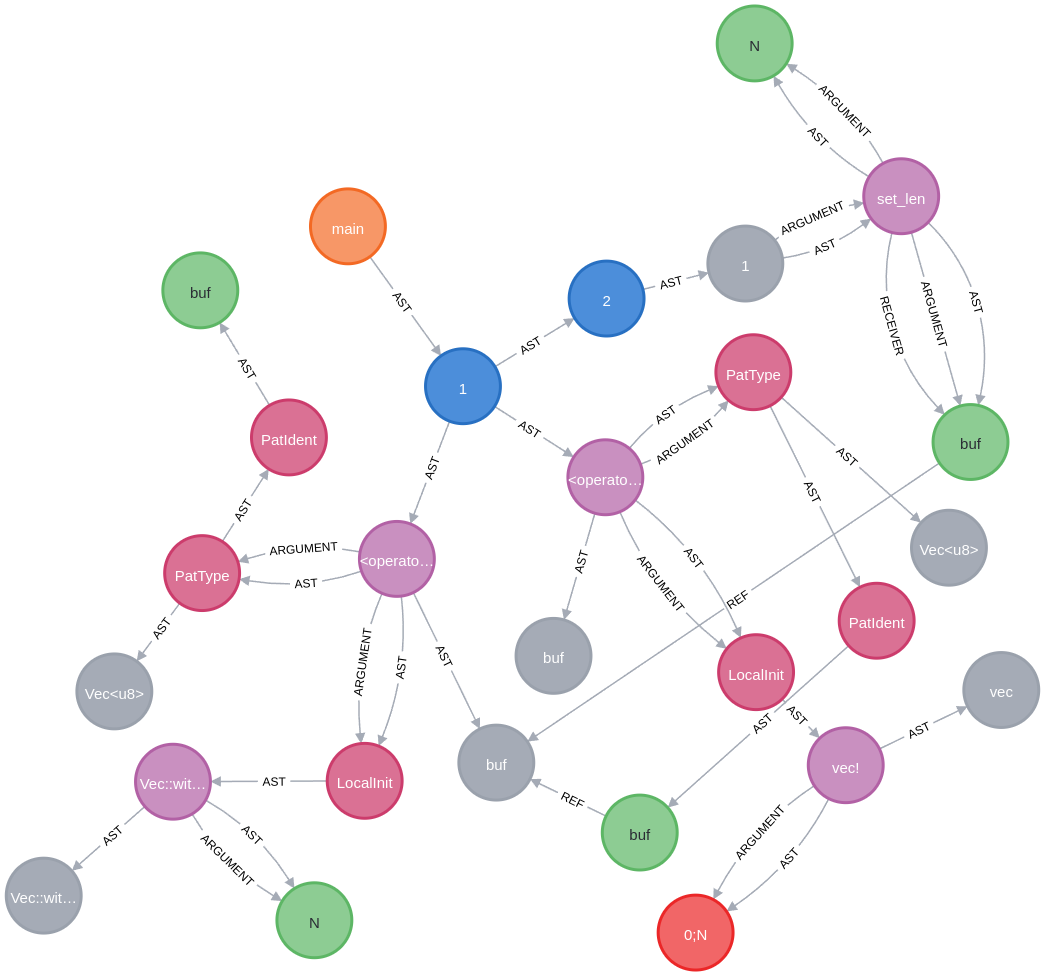
\includegraphics[width=1\columnwidth]{figures/c4/c4_RUSTSEC-2021-0086}
    \centering
    \caption{Ví dụ đồ thị CPG cho đoạn mã nguồn RUSTSEC-2021-0086 \ref{code:c4_RUSTSEC-2021-0086}}
    \label{img:c4_RUSTSEC-2021-0086}
\end{figure}

\subsection{RUSTSEC-2022-0028}

Lỗi RUSTSEC-2022-0028 xảy ra khi sử dụng hàm \texttt{external} mà không xác dịnh đúng ràng buộc lifetime cho kiểu tổng quát \texttt{T}.
Trong bối cảnh này, \texttt{ArrayBuffer} là hàm được dùng để giao tiếp giữa Rust và Javascript thông qua Web Assembly Binding \cite{ githubGitHubRustwasmwasmbindgen}.
Điều này cho phép tạo ra một \texttt{ArrayBuffer} từ các kiểu dữ liệu có thể bị giải phóng trong khi chúng vẫn được tham chiếu bởi \texttt{ArrayBuffer} trong Javascript.
Để sửa lỗi, cần thêm ràng buộc \texttt{T: 'static} để đảm bảo rằng dữ liệu được tham chiếu sẽ không bị giải phóng trong suốt thời gian tồn tại của \texttt{ArrayBuffer}.

\begin{listing}[H]
\begin{minted}[mathescape, breaklines, frame=lines, framesep=2mm, baselinestretch=1.2, fontsize=\footnotesize, linenos]{rust}
// Before fix
pub fn external<'a, C, T>(cx: &mut C, data: T) -> Handle<'a, Self>
where
    C: Context<'a>,
    T: AsMut<[u8]> + Send,
{
    // ...
}

// After fix
pub fn external<'a, C, T>(cx: &mut C, data: T) -> Handle<'a, Self>
where
    C: Context<'a>,
    T: AsMut<[u8]> + Send + 'static,
{
    // ...
}
\end{minted}
\caption{Ví dụ mã nguồn cho RUSTSEC-2022-0028}
\label{code:c4_RUSTSEC-2022-0028}
\end{listing}

\begin{figure}[H]
    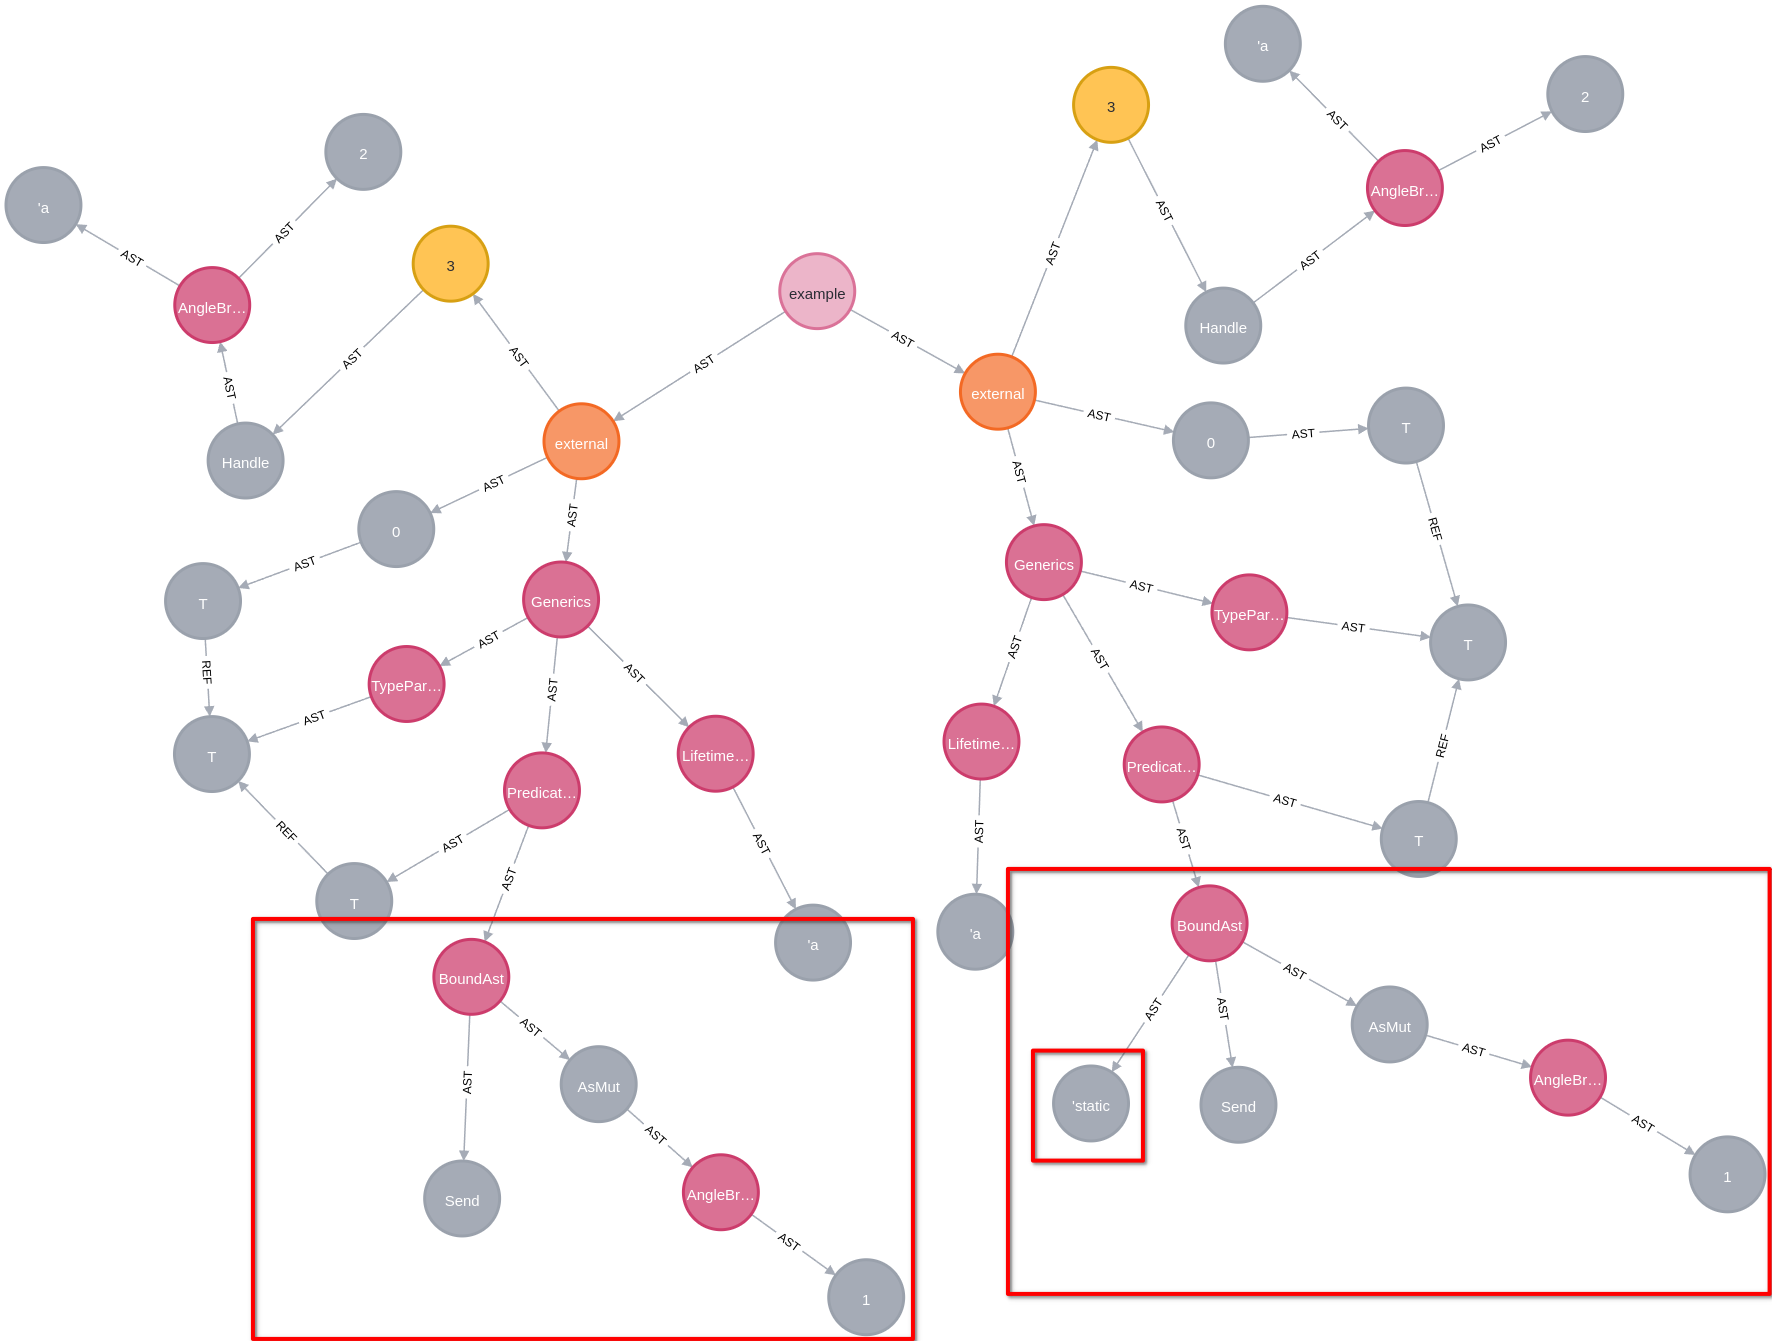
\includegraphics[width=1\columnwidth]{figures/c4/c4_RUSTSEC-2022-0028.png}
    \centering
    \caption{Ví dụ đồ thị CPG cho đoạn mã nguồn RUSTSEC-2022-0028 \ref{code:c4_RUSTSEC-2022-0028}}
    \label{img:c4_RUSTSEC-2022-0028}
\end{figure}

\subsection{RUSTSEC-2020-0044}

RUSTSEC-2020-0044 là lỗi liên quan đến việc không triển khai \texttt{trait Send} cho kiểu dữ liệu con của kiểu \texttt{Atom}.
Trong bối cảnh này, \texttt{Atom} đóng vai trò như một "hộp" cho kiểu dữ liệu \texttt{P} bên trong, giúp quản lý việc sử dụng bộ nhớ an toàn hơn.
Tuy nhiên chỉ mình \texttt{Atom} được cài đặt \texttt{trait Send} và \texttt{Sync}, không đảm bảo rằng kiểu dữ liệu con \texttt{P} cũng phải cài đặt \texttt{trait Send}.
Điều này có nghĩa việc truy cập đến \texttt{Atom} có thể an toàn nhưng khi truy cập vào dữ liệu kiểu \texttt{P} bên trong thì không an toàn, có thể dẫn đến các vấn đề như sử dụng bộ nhớ sau khi đã giải phóng hoặc tương tranh dữ liệu cho kiểu dữ liệu \texttt{P} bên trong.
Để sửa lỗi này, cần đảm bảo rằng kiểu \texttt{P} cũng phải được đánh dấu \texttt{trait Send}.
Điều này có nghĩa là nếu kiểu cha muốn được gửi qua các luồng một cách an toàn bằng \texttt{trait Send} thì kiểu con \texttt{P} cũng phải có khả năng này, tương tự với trait \texttt{Sync}.

\begin{listing}[H]
\begin{minted}[mathescape, breaklines, frame=lines, framesep=2mm, baselinestretch=1.2, fontsize=\footnotesize, linenos]{rust}
// Before fix
unsafe impl<P> Send for Atom<P> where P: IntoRawPtr + FromRawPtr {}
unsafe impl<P> Sync for Atom<P> where P: IntoRawPtr + FromRawPtr {}

// After fix
unsafe impl<P> Send for Atom<P> where P: IntoRawPtr + FromRawPtr + Send {}
unsafe impl<P> Sync for Atom<P> where P: IntoRawPtr + FromRawPtr + Send {}
\end{minted}
\caption{Ví dụ mã nguồn cho RUSTSEC-2020-0044}
\label{code:c4_RUSTSEC-2020-0044}
\end{listing}

\begin{figure}[H]
    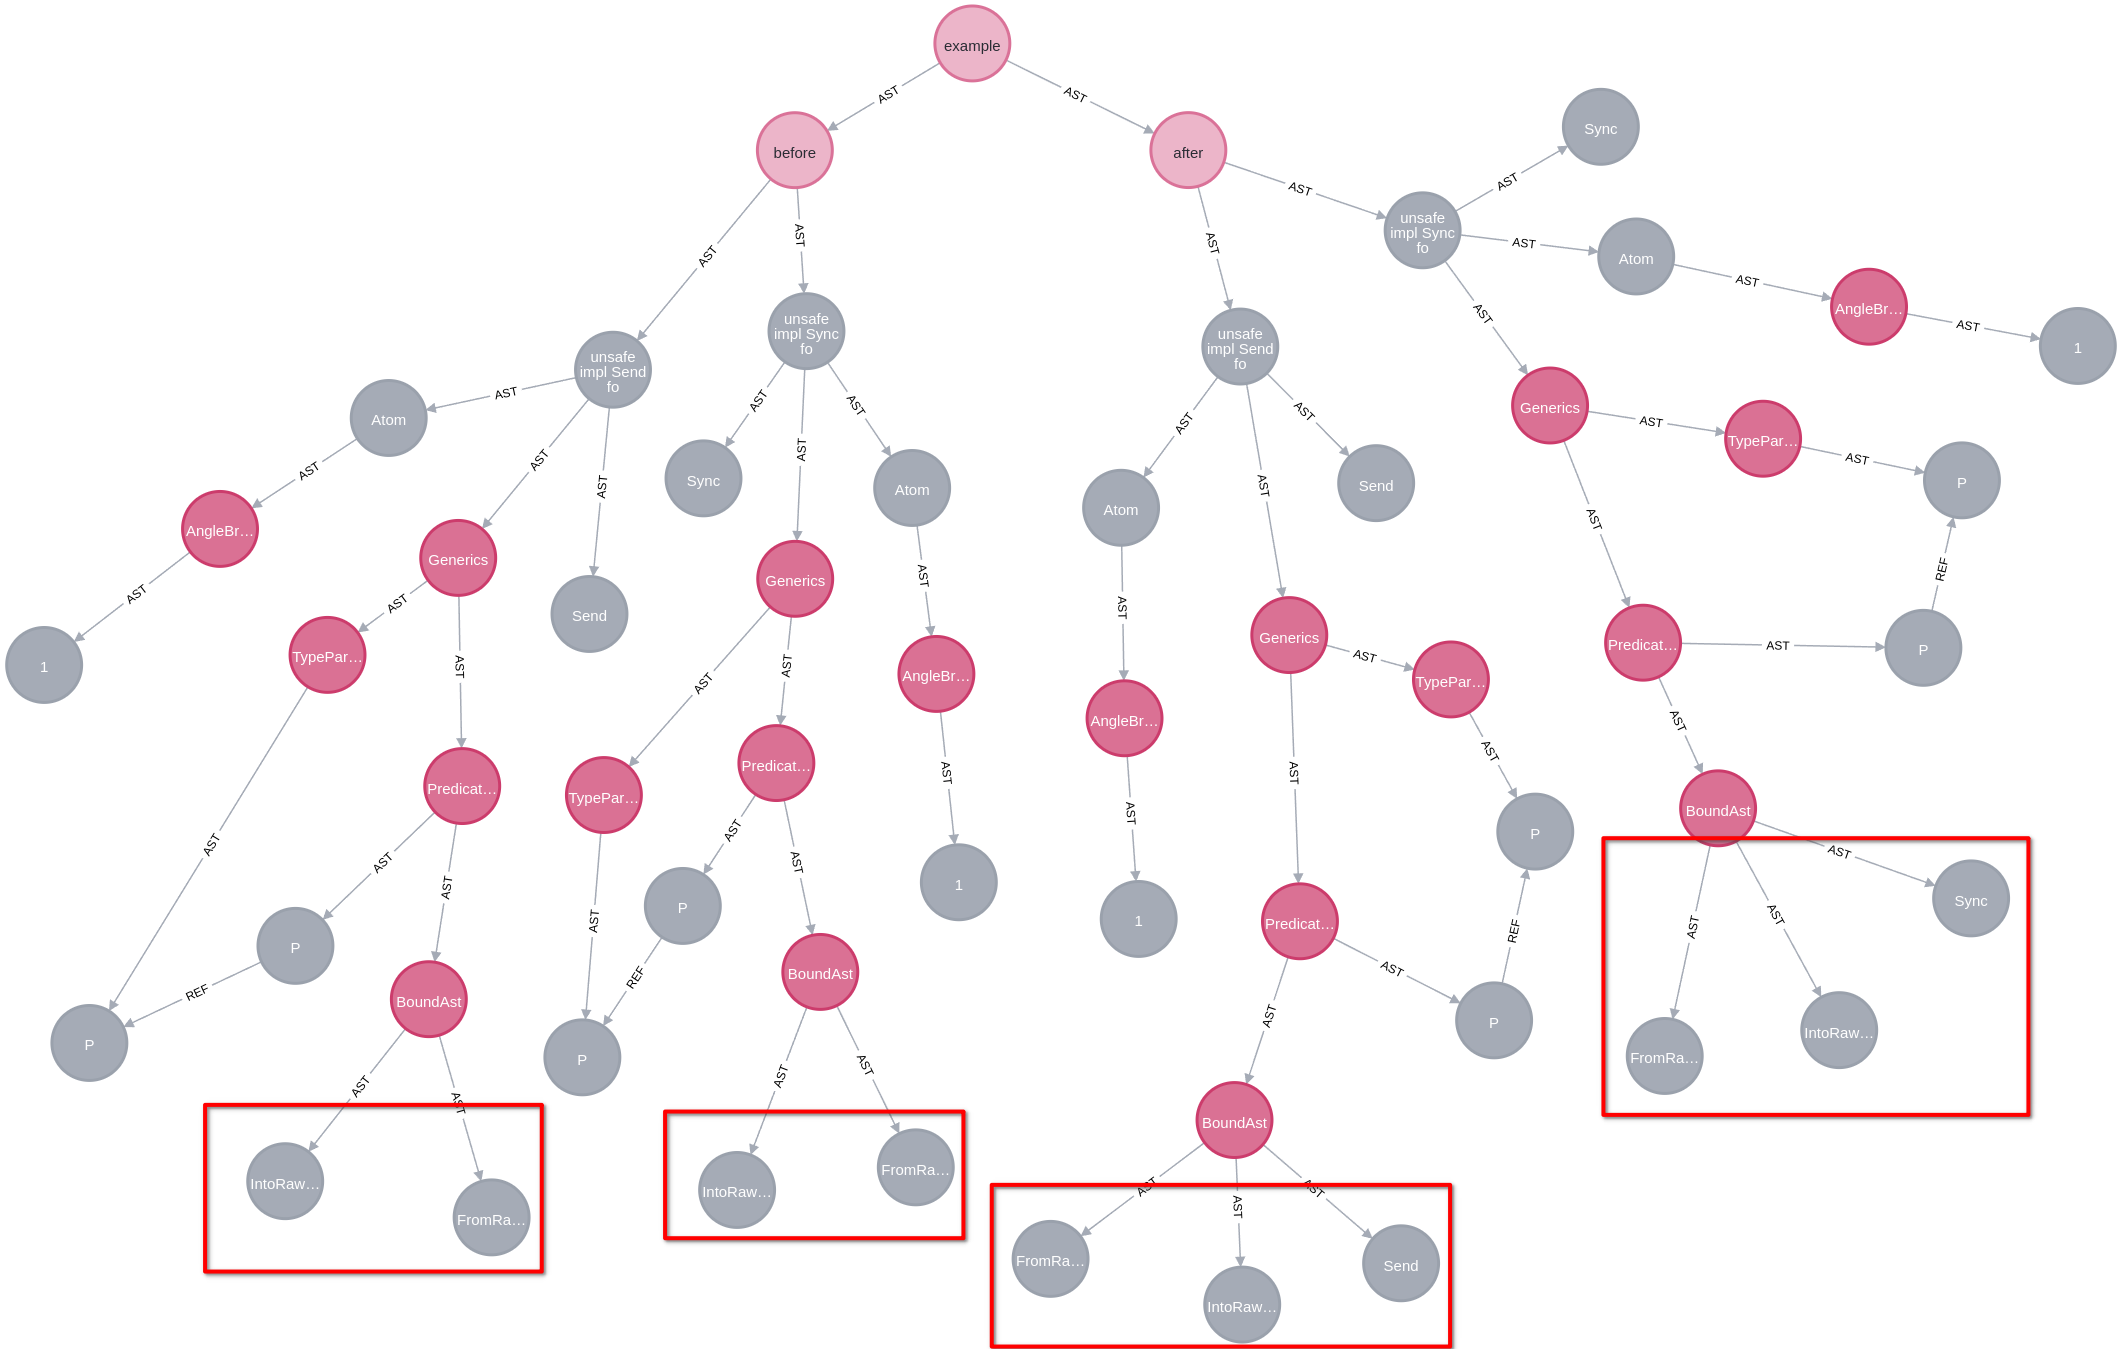
\includegraphics[width=1\columnwidth]{figures/c4/c4_RUSTSEC-2020-0044.png}
    \centering
    \caption{Ví dụ đồ thị CPG cho đoạn mã nguồn RUSTSEC-2020-0044 \ref{code:c4_RUSTSEC-2020-0044}}
    \label{img:c4_RUSTSEC-2020-0044}
\end{figure}

Kiểu cha muốn đảm bảo an toàn về đa luồng thì kiểu con cũng phải đảm bảo an toàn về đa luồng.
Đây là một mẫu có thể được xây dựng và áp dụng cho nhiều đoạn mã khác.
Các truy vấn hoặc phân tích dựa trên mẫu này có thể được áp dụng trên đồ thị CPG để phát hiện các lỗi tương tự.

\subsection{RUSTSEC-2021-0130}

RUSTSEC-2021-0130 là lỗi về sử dụng bộ nhớ sau khi đã giải phóng.
Trong bối cảnh này, \texttt{Iter} là một \texttt{struct} được sử dụng để duyệt qua các phần tử trong một danh sách liên kết.
Tuy nhiên, khi \texttt{Iter} được trả về từ hàm \texttt{iter} thì nó sẽ trỏ tới \texttt{self.head} mà \texttt{self.head} có thể bị giải phóng trước khi \texttt{Iter} được sử dụng, dẫn đến việc sử dụng bộ nhớ sau khi đã giải phóng.
Nguyên nhân là do quan hệ lifetime giữa biến \texttt{self} và giá trị trả về kiểu \texttt{Iter} không đồng bộ.
Biến \texttt{self} được chỉ định lifetime là \texttt{'\_}, tức là để trình biên dịch tự gán một giá trị lifetime mặc định, trong khi đó kiểu trả về \texttt{Iter} được chỉ định lifetime là \texttt{'a}.
Trong trường hợp này \texttt{'\_} và \texttt{'a} không có liên hệ với nhau do đó lifetime của \texttt{Iter} có thể lớn hơn lifetime của \texttt{self}, dẫn đến việc truy cập đến \texttt{self.head} sau khi \texttt{self} đã bị giải phóng.
Để sửa lỗi, cần sử dụng cùng chung một lifetime cho \texttt{self} và \texttt{Iter} thông qua việc sử dụng quy tắc 3 của lifetime ellision.
Nếu không chỉ định lifetime một cách tường minh, ba quy tắc lifetime ellision sẽ được trình biên dịch sử dụng để tự động xác định lifetime của các biến dựa trên cấu trúc của hàm, bao gồm:

\begin{enumerate}
    \item Mỗi tham số kiểu tham chiếu của hàm mặc định có một lifetime riêng.
    \item Khi hàm có một tham số duy nhất kiểu tham chiếu, và kiểu trả về cũng là kiểu tham chiếu thì lifetime của kiểu trả về sẽ là lifetime của tham số duy nhất đó.
    \item Nếu hàm có nhiều tham số kiểu tham chiếu nhưng có một tham số là \texttt{self} (\texttt{self} tương đương với \texttt{this} trong C++ và Java), thì lifetime của \texttt{self} sẽ được gán cho kiểu tham số trả về.
\end{enumerate}

Trong trường hợp này sửa lỗi bằng cách không chỉ định lifetime cho \texttt{self} mà để trình biên dịch tự xác định, lifetime của \texttt{Iter} sẽ để là \texttt{'\_}, tức là tự động suy diễn và áp dụng quy tắc 3 của lifetime ellision thì lifetime của \texttt{Iter} sẽ được gán bằng lifetime của \texttt{self}.
Từ đó lifetime của \texttt{Iter} sẽ không lớn hơn lifetime của \texttt{self} và việc truy cập đến \texttt{self.head} sau khi \texttt{self} đã bị giải phóng sẽ không xảy ra.

\begin{listing}[H]
\begin{minted}[mathescape, breaklines, frame=lines, framesep=2mm, baselinestretch=1.2, fontsize=\footnotesize, linenos]{rust}
// Before fix
pub fn iter<'a>(&'_ self) -> Iter<'a, K, V> {
    Iter { ptr: unsafe { (*self.head).next }, }
}

// After fix
pub fn iter(&self) -> Iter<'_, K, V> {
    Iter { ptr: unsafe { (*self.head).next }, }
}
\end{minted}
\caption{Ví dụ mã nguồn cho RUSTSEC-2021-0130}
\label{code:c4_RUSTSEC-2021-0130}
\end{listing}

\begin{figure}[H]
    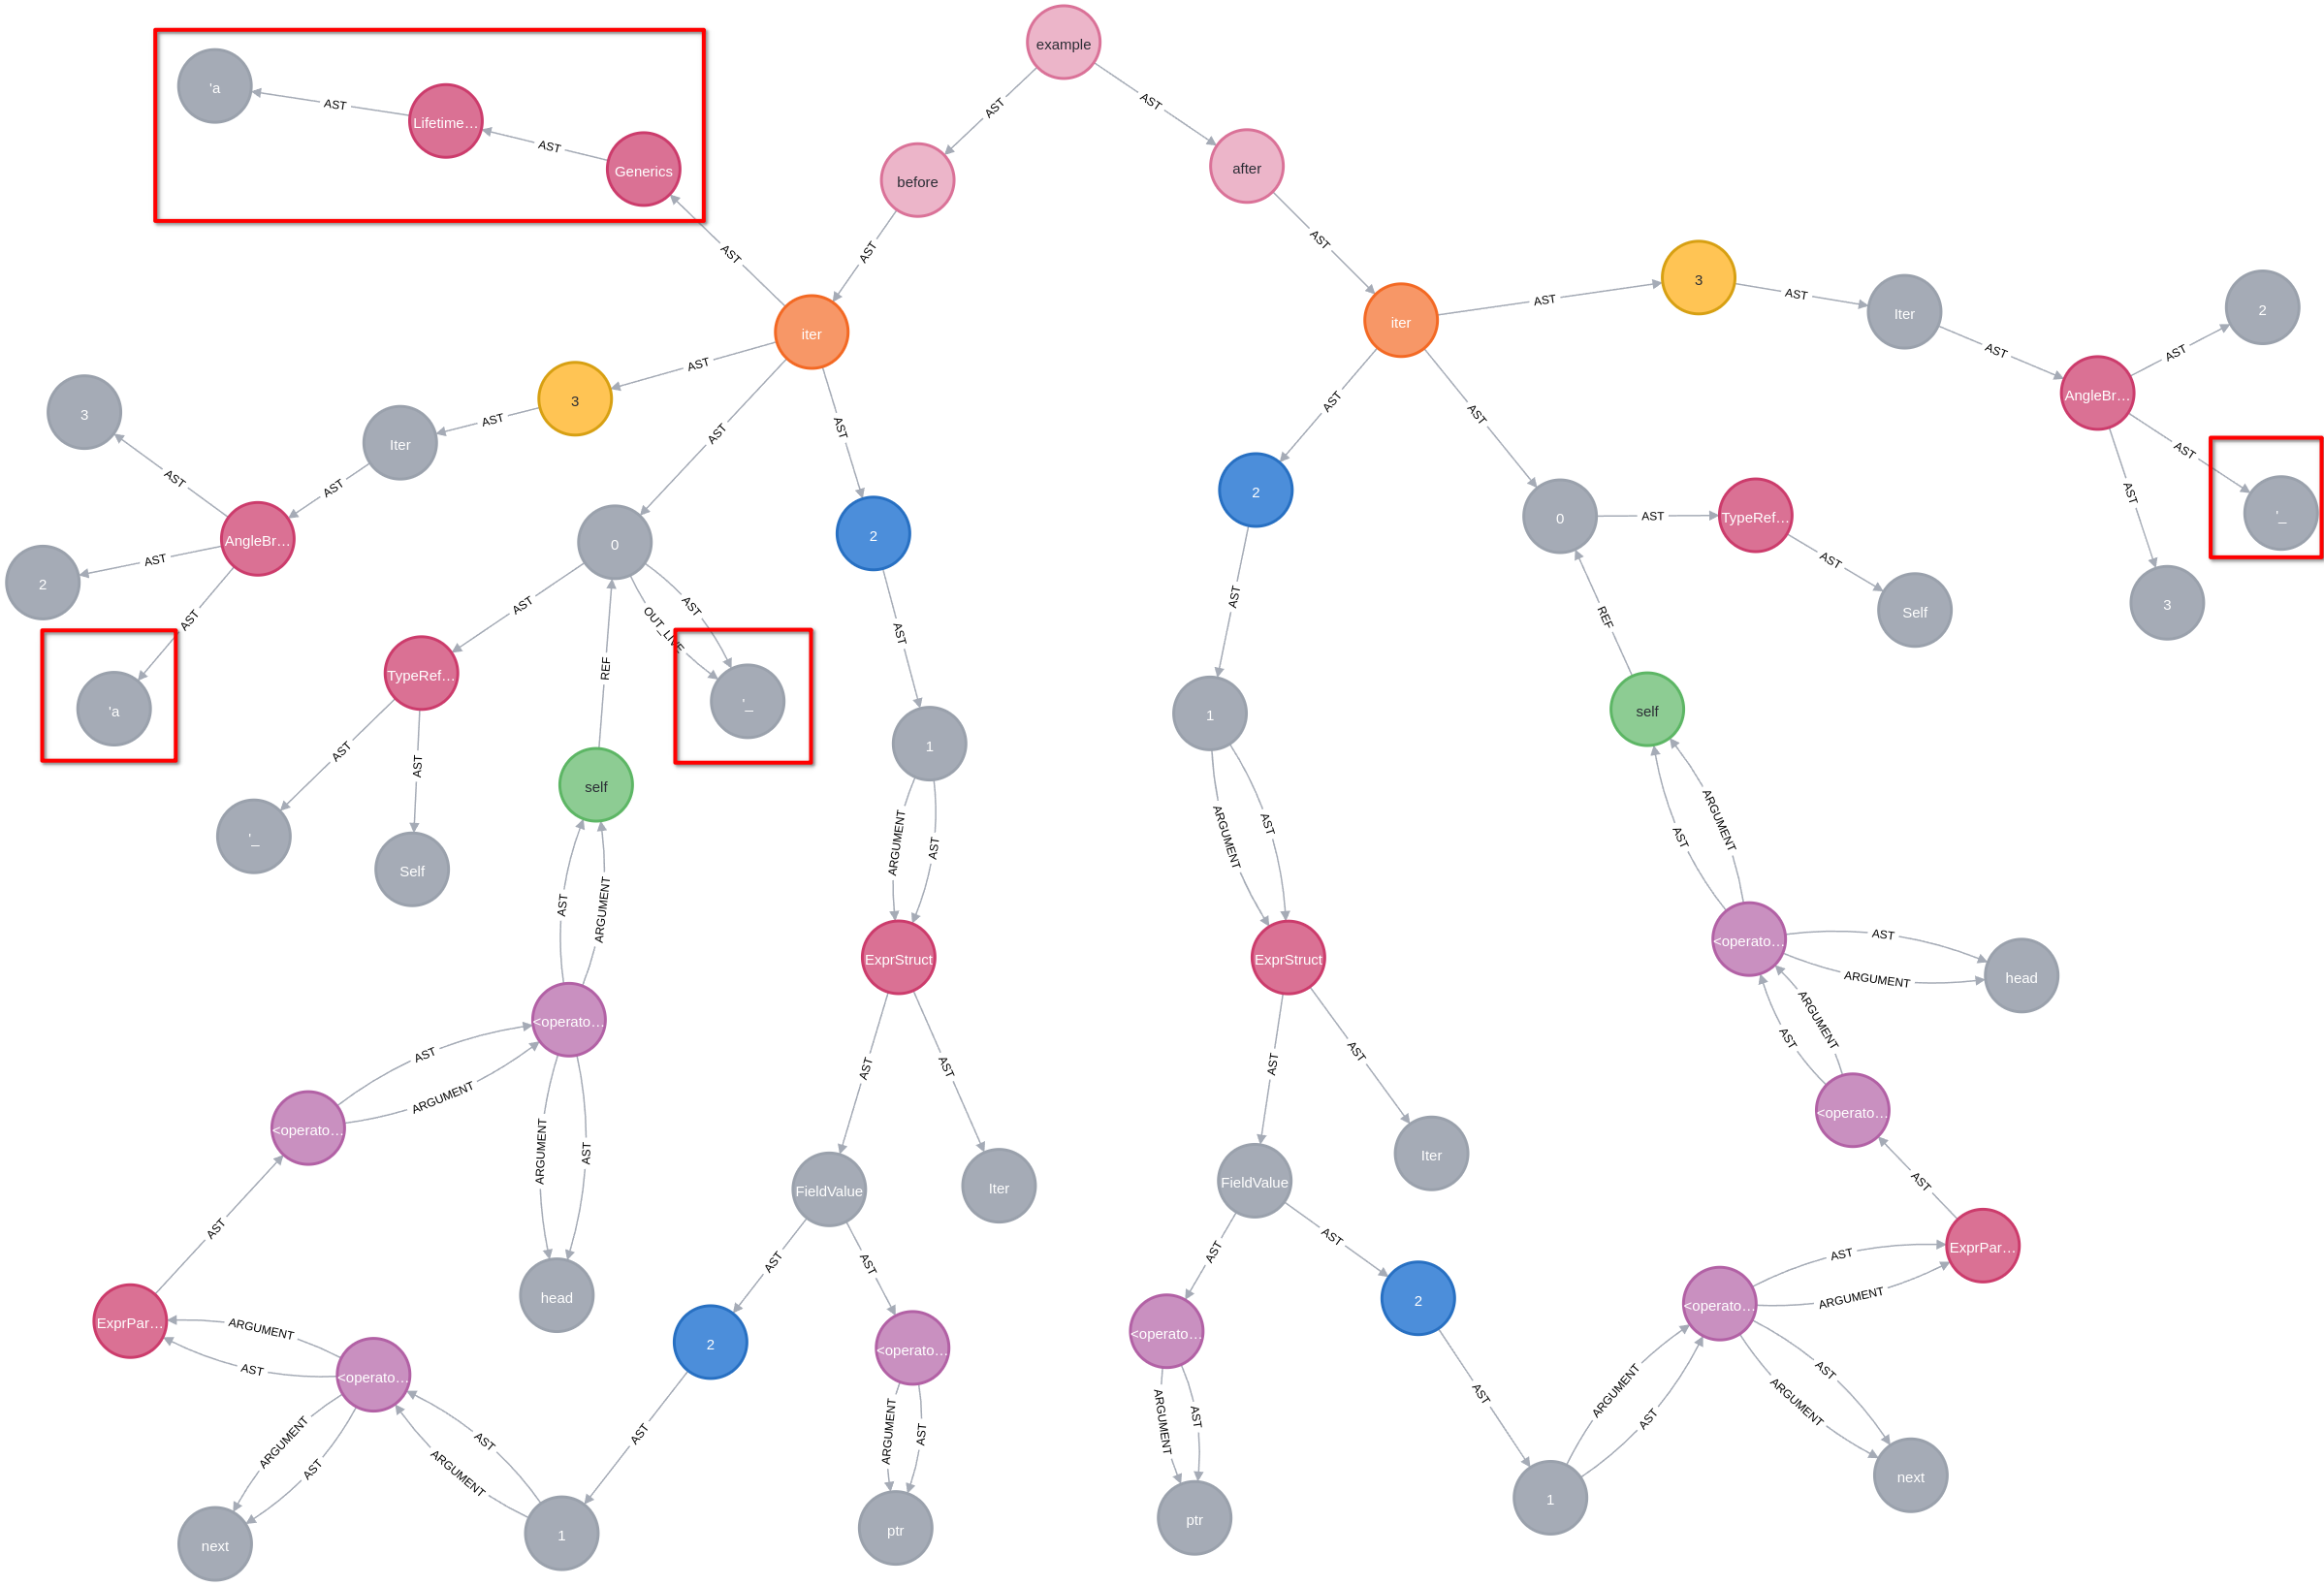
\includegraphics[width=1\columnwidth]{figures/c4/c4_RUSTSEC-2021-0130.png}
    \centering
    \caption{Ví dụ đồ thị CPG cho đoạn mã nguồn RUSTSEC-2021-0130 \ref{code:c4_RUSTSEC-2021-0130}}
    \label{img:c4_RUSTSEC-2021-0130}
\end{figure}

Đánh dấu lifetime một cách tường minh cần được thực hiện cẩn thận để tránh được các lỗi liên quan đến bộ nhớ.
Việc đánh dấu lifetime không chính xác có thể đánh lừa trình biên dịch và dẫn đến việc sử dụng bộ nhớ sau khi đã giải phóng.
Lifetime của kiểu trả về phải đảm bảo không lớn hơn lifetime của tham số truyền vào nếu kiểu trả về có truy cập đến bộ nhớ của tham số truyền vào.
Có thể áp dụng các quy tắc lifetime ellision để suy diễn việc xác định lifetime giữa tham số và tham số, giữa tham số và kiểu trả về.
Các luật có thể được đề ra để phát hiện sự không đồng bộ về lifetime giữa các biến, từ đó giúp phát hiện lỗi về bộ nhớ trên đồ thị CPG.
